\documentclass[../jaynes_prob_theory_notes.tex]{subfiles}
%\usepackage[margin=1in]{geometry}
%\usepackage{amsmath}
%\usepackage{graphicx}

\begin{document}

\section{Elementary sampling theory}
Recall the basic rules:
    \begin{itemize}
        \item Product: $P(AB|C) = P(A|BC)P(B|C) = P(B|AC)P(A|C)$
        \item Sum: $P(AB) + P(\bar{A}|B) = 1$
        \item Extended sum: $P(A + B|C) = P(A|C) + P(B|C) - P(AB|C)$
        \item Principle of indifference: $P(H_i|B) = 1/N$, $1 \leq i \leq N$
          - iff the set $H_i$ is exhaustive and mutually exclusive
        \item Bernoulli urn rule: $P(A|B) = M/N$
          - iff B specifies that A is true on some subset of $H_i$ and false on the remaining $N-M$ 
    \end{itemize}
    
\subsection{Sampling without replacement}
    EXAMPLE: Bernoulli urn reexamined
        \begin{itemize}
            \item Propositions
                \begin{enumerate}
                    \item $B \equiv$ An urn contains $N$ balls, identical except that they are labeled sequentially and $M$ of them are coloured red, with the remaining $N-M$ coloured white. We draw a ball, observe and record its colour, and do not replace it. This is done until $n$ balls are drawn, $0 \leq n \leq N$
                    \item $R_i \equiv$ Red ball on the $i$th draw
                    \item $W_i \equiv$ White ball on the $i$th draw
                \end{enumerate}
        
            \item Since only red or white can be drawn, we know that $P(R_i|B) + P(W_i|B) = 1$
            \item The propositions are related by the negations $\bar{R}_i = W_i$ and $R_i = \bar{W}_i$
            \item So, the first draw is then defined by the probabilities: $P(R_1|B) = M/N$ and $P(W_1|B) = 1 - M/N$
            \item Subsequent draws can be derived from the product rule: $P(R_1R_2|B) = P(R_1|B)P(R_2|B)$, but need to take into account that the ball being drawn is not replaced. 
                \begin{itemize}
                    \item Therefore, $P(R_1R_2|B) = \frac{M}{N}\frac{M-1}{N-1}$
                    \item can be extended to $r$ draws: $P(R_1R_2 \ldots R_r|B) = \frac{M!(N-r)!}{(M-r)!N!}$, where $r \leq M$ 
                \end{itemize}
        
            \item What is the probabiltiy of drawing exactly $r$ red balls in $n$ draws, regardless of order?
                \begin{itemize}
                    \item must multiply by the bionomial coefficient: $\binom{n}{r} = \frac{n!}{r!(n-r)!}$, which represents the number of possible orders of drawing $r$ red balls in $n$ draws, called the multiplicity of the event $r$.
                        \begin{itemize}
                            \item for example, to get three red in three draws, $\binom{3}{3} = 1$, can only happen in one way, $R_1R_2R_3$
                            \item However, to get two red in three draws, $\binom{3}{2} = 3$, can happen in three ways, $R_1R_2W_3$, $R_1W_2R_3$, and $W_1R_2R_3$.
                        \end{itemize}
                    \item We can then derive an expression for drawing exactly $R$ red balls in $n$ draws, defined by the function $h(r|N, M, n) \equiv P(A|B)$
                        \begin{itemize}
                            \item[] $h(r|N, M, n) = \frac{\binom{M}{r}\binom{N-M}{n-r}}{\binom{N}{n}}$
                            \item This is called the hypergeometric distribution, often abbreviated as $h(r)$
                        \end{itemize}
                    \item it can be demonstrated that the hypergeometric distribution is symmetric on exchange of $M$ and $n$, i.e. $h(r|N, M, n) = h(r|N, n, M)$. So, the probability of drawing ten ball balls from an urn containing 50 red ones is the same as drawing 50 balls from an urn containing 10 red ones.
                    \item generalized hypergeometric distribution: 
                        \begin{equation*}
                        h(r_1\ldots r_k|N_1\ldots N_k) = \frac{\binom{N_1}{r_1} \ldots \binom{N_k}{r_k}}{\binom{\sum N_i}{\sum r_i}}
                        \end{equation*}
                        where there are $k$ different colours of $N$ balls, drawn $n = \sum r_i$ times
                \end{itemize}
            \item we can find the most probable value of $r$ by setting $h(r^{\prime}) = h(r^{\prime} - 1)$, and solving for $r^{\prime}$. (this makes sense if you think about it like a distribution with a peak)
            \item the width of the distribution $h(r)$ gives an indication of the accuracy with which we can predict $r$
            \item Cumulative probability distribution: $H(R) \equiv \sum^{R}_{r=0}h(r)$, which is the probability of finding $R$ or fewer red balls
                \begin{itemize}
                    \item $H(R)$ is a step function (think the first term in your first project)
                \end{itemize}
            \item the median of the probability function is defined to be a numer $m$ which has equal probabilities associated with $(r < m)$ and $(r > m)$ (think a transition state)
        
            \item What is the probability of drawing a red ball on the second draw, $P(R_2|B)$, without knowledge of the first draw's result?
                \begin{itemize}
                    \item we know that either $R_1$ or $W_1$ is true, so $R_2 = (R_1 + W_1)R_2 = R_1R_2 + W_1R_2$
                    \item applying the product rule, we get 
                        \begin{equation*}
                        P(R_2|B) = P(R_1R_2|B) + P(W_1R_2|B) = P(R_2|R_1B)P(R_1|B) + P(R_2|W_1B)P(W_1|B)
                        \end{equation*}
                    \item but $P(R_2|R_1B) = \frac{M-1}{N-1}$ and $P(R_2|W_1B) = \frac{M}{N-1}$
                    \item so $P(R_2|B) = \frac{M-1}{N-1}\frac{M}{N} + \frac{M}{N-1}\frac{N-M}{N} = \frac{M}{N}$
                    \item notice that everything cancels out such that we have the same probability for red on the first and second draws.
                    \item this holds true generally, so the probability to draw red at any draw is the same, iff we do not know the result of any other draw
                \end{itemize}
        \end{itemize}

\subsection{Logic vs Propensity}
    \begin{itemize}
        \item since we know that knowledge of a earlier drawn ball's colour  can change the probability of the current draw, can knowledge of a future ball's colour change the probability of the current ball?
        \item usually a fundamental axiom that future events can't change the probability of a current event
        \item but lets say we have an urn with two balls, one red and one white.\ the probability to draw a white ball with priors B is $P(W_1|B) = 1/2$. But what if we knew that the second draw was red? Then the probability becomes unity ($P(W_1|B) = 1$).
        \item So, while information about a later draw does not change the physical nature of the system, i.e.\ it does not change the number of balls of each colour in the system, it does change the state of knowledge of the system in the same way that knowledge of a past draw would
        \item this suggests that logical inference is fundamentally different from physical causation, e.g.\ physical influences propagate only forward in time while logical inferences propagate equally in either direction
        \item if the probability of an event is invariant under an permutation of the events (e.g.\ when the event took place), the probability distribution is called exchangeable.\ the hypergeometric distribution discussed above in the Bernoulli's urn example is exchangeable
    \end{itemize}
    
\subsection{Expectations}
    \begin{itemize}
        \item definition: if a variable $x$ can take on the set of values $(x_1, \ldots, x_n)$, in $n$ mutually exclusive and exhaustive situations, and we assign probabilities $(p_1, \ldots, p_n)$, the quantity $\langle x \rangle = E(x) = \sum^n_{i=1}p_ix_i$ is the expectation balue of $x$
            \begin{itemize}
                \item (you know this from quantum mechanics)
                \item it is a weighted average of the possible values of $x$, weighted by their corresponding probabilities
            \end{itemize}
        \item this brings us to a an easier way to discuss probabilities with prior knowledge of an event at some later time not known
            \begin{itemize}
                \item if $F = M/N$ of red balls is known, then $P(R_1|B) = F$
                \item if $F$ is unknown, $P(R_1|B) = \langle F \rangle$
            \end{itemize}
    \end{itemize}
    
    \subsection{Binomial Distribution}
        \begin{itemize}
            \item the hypergeometric distribution takes into account the changing nature of the urn, i.e.\ drawing a ball changes the contents to N-1. 
            \item but what if $N \gg n$? the probability  changes very little, and in the limit $N \rightarrow \infty$, this becomes negligible
            \item thus the hypergeometric distribution simplifies to the binomial distribution (through a derivation i don't care to type):
                \begin{itemize}
                    \item[] $h(r|N, M, n) \rightarrow b(r|n, f) \equiv \binom{n}{r}f^r(1-f)^{n-r}$ where $M/N \rightarrow f$
                \end{itemize}
        \begin{figure*}[h!]
            \centering
            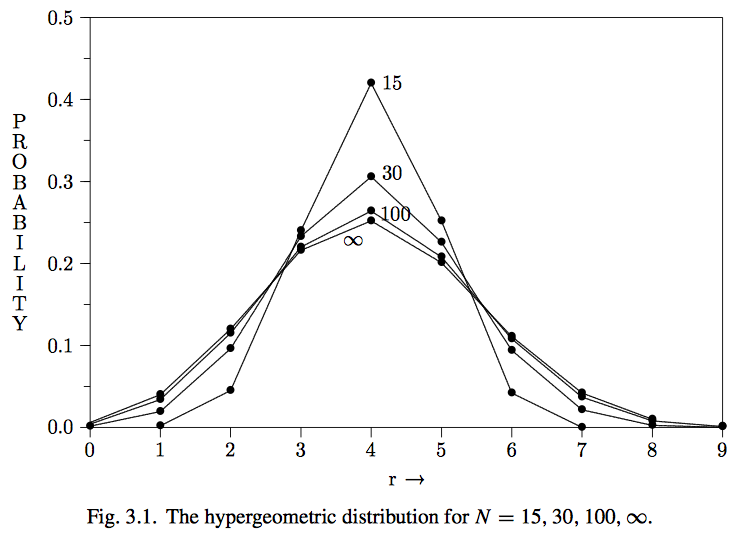
\includegraphics[width=0.5\textwidth]{binom.png}
            \caption{Comparing the hypergeometric distribution to the binomial distribution (the hypergeometric distribution in the $N \rightarrow \infty$ limit}
        \end{figure*}
        
            \item another limiting case, where $N_i \rightarrow \infty$, in such a way that $f_i \equiv \frac{N_i}{\sum N_j} =$ constant,
                \begin{itemize}
                    \item[] $m(r_1\ldots r_k|f_1\ldots f_k) = \frac{r!}{r_1! \ldots r_k!}f_1^{r_1}\ldots f_k^{r_k}$ where $r\equiv \sum r_i$
                    \item this is called the multinomial distribution
                \end{itemize}
        \end{itemize}

\subsection{Sampling with replacement}
    \begin{itemize}
        \item suppose instead of placing a drawn ball to the side, we instead put it back into the urn?
        \item with background information $B^{\prime}$, the probability of drawing two red balls in succession is $P(R_1R_2|B^{\prime}) = P(R_1|B^{\prime})P(R_2|R_1B^{\prime})$
            \begin{itemize}
                \item clearly the first factor, $P(R_1|B^{\prime})$ is still $M/N$, but what about the second factor?
                \item (there is an interesting digression on reality vs models wrt randomization, on pp. 73-75. randomization is not truly something found in nature, what we mean by randomization is that no human is able to implicitly or explicitly influence the results)
                \item if we assume the urn to be randomized upon replacement, information of $R_1$ is irrelevant to draw 2, so $P(R_2|R_1B^{\prime}) = P(R_2|B^{\prime}) = M/N$. this holds true generally for any draw.
                \item the probability for drawing exactly $r$ balls in $n$ trials is simply $\binom{n}{r}\left(\frac{M}{N}\right)^r\left(\frac{N-M}{N}\right)^{n-r}$, which is just the binomial distribution
                \item thus, the probability of drawing $r$ red balls with replacement is the same as drawing $r$ red balls without replacement in the limit $N \rightarrow \infty$
                \item this approximation, however, can accumulate errors for large $n$
                    \begin{itemize}
                        \item suppose that drawing and replacing a red ball increases the probability of drawing a red ball on the next draw by some small amount $\epsilon > 0$, while drawing a white ball decreases it by some small amount $\delta > 0$ (think of this as nonoptimal shaking of the urn)
                        \item letting $C$ be the background information described above, we have the following probabilities: 
                            \begin{align*}
                                P(R_k|R_{k-1}C) &= p + \epsilon & P(R_k|W_{k-1}C) &= p - \delta \\
                                P(W_k|R_{k-1}C) &= 1 - p - \epsilon & P(W_k|W_{k-1}C) &= 1 - p + \delta
                            \end{align*}
                            where $p \equiv M/N$ (this is referenced below)
                        \item from this, the probability of drawing $r$ red balls and $(n-r)$ white balls in any order is $p(p+\epsilon)^c(p-\delta)^{c^{\prime}}(1-p+\delta)^w(1-p-\epsilon)^{w^{\prime}}$, where $c$ is the number of red draws preceded by red ones, $c^{\prime}$ is the number of red preceded by white, $w$ is the number of white preceded by white, and $w^{\prime}$ is the number of white preceded by red.
                        \item we can additionally see that $c+c^{\prime} = \left[\begin{smallmatrix}r-1\\r\end{smallmatrix}\right]$ and $w + w^{\prime} = \left[\begin{smallmatrix} n-r \\ n-r-1 \end{smallmatrix}\right]$, where the upper and lower cases are when the first draw is red or white, respectively.
                            \begin{itemize}
                                \item when $r$ and $(n-r)$ are small, $\epsilon$ and $\delta$ are negligible, and the expression simplifies to $p^r(1-p)^{n-r}$, as in the binomial distribution above
                                \item but as $r, n \rightarrow \infty$, we can use the relation $\left(1+\frac{\epsilon}{p}\right)^c \approx \mathrm{exp} \left(\frac{\epsilon c}{p}\right)$, so that the probability goes to $p^r(1-p)^{n-r}exp\left(\frac{\epsilon c - \delta c^{\prime}}{p} + \frac{\delta w - \epsilon w^{\prime}}{1-p}\right)$
                                \item thus, the probability now depends on the order, and depending on $\epsilon$ and $\delta$, the deviation from the binomial distribution can be large
                            \end{itemize}
                    \end{itemize}
                \item Let's see how this affects previous calculations
                    \begin{itemize}
                        \item for the first draw we still have $p = P(R_1|C) = M/N$ and $q = 1 - p = P(W_1|C) = \frac{N-M}{N}$
                        \item but for the second trial we have $P(R_2|C) = p + (p\epsilon - q\delta)$, and $P(R_3|C) = p + (1+\epsilon + \delta)(p\epsilon - q\delta)$ for the third. does $P(R_k|C)$ approach some limit as $k \rightarrow \infty$?
                        \item if we write the probabilities for the $k$th trial as a vector $V_k \equiv \left[\begin{smallmatrix} P(R_k|C) \\ P(W_k|C) \end{smallmatrix}\right]$, the set of the four probabilites above can be written in matrix form $V_k = MV_{k-1}$ where $M = \left[ \begin{smallmatrix} p+\epsilon & p-\delta \\ q-\epsilon & q+\delta \end{smallmatrix} \right]$
                            \begin{itemize}
                                \item This is a Markov chain of probabilities (!), and $M$ is called the transition matrix. 
                                \item So draws after the first can be expressed like $V_k = M^{k-1}V_1$. 
                                \item To find a general solution, we need to find the eigenvectors and eigenvalues of $M$: $C(\lambda) \equiv \mathrm{det}(M_{ij} - \lambda\delta_{ij}) = \lambda^2 - \lambda(1+\epsilon+\delta)+(\epsilon+\delta)$, so $\lambda_1=1$ and $\lambda_2 = \epsilon + \delta$
                                \item the eigenvectors are $x_1 = \binom{p-\delta}{q-\epsilon}$ and $x_2 = \binom{1}{-1}$, which are not orthogonal.
                                \item using these to define the transition matrix, $S = \left( \begin{smallmatrix} p-\delta & 1 \\ q-\epsilon & -1 \end{smallmatrix} \right)$, we can diagonalize $M$, $(S^{-1} M S)$, to eventually get to the general solution: 
                                    \begin{equation*}
                                    P(R_k|C) = \frac{(p-\delta)-(\epsilon+\delta)^{k-1}(p\epsilon-q\delta)}{1-\epsilon-\delta}
                                    \end{equation*}
                                \item when $\epsilon = \delta = 0$, this simplifies to $P(R_k|C) = p$
                            \end{itemize}
                        \item interesting to note that $\epsilon + \delta = 1$ iff $\epsilon = q$ and $\delta = p$ (since $0 \leq p \leq 1$, $\epsilon$ and $\delta$ must be bounded to the interval [-1,1]), the transition matrix simplifies to $M=\left[ \begin{smallmatrix} p+\epsilon & p-\delta \\ q-\epsilon & q+\delta \end{smallmatrix} \right] = \left(\begin{smallmatrix} 1 & 0 \\ 0 & 1 \end{smallmatrix} \right)$, and no transitions occur
                        \item likewise, if $\epsilon + \delta = -1$, $M = \left(\begin{smallmatrix} 0 & 1 \\ 1 & 0 \end{smallmatrix} \right)$, and nothing but transitions occur, i.e. colours alternate after the first draw
                        \item in the realistic case where $0 < |\epsilon + \delta| < 1$, the general solution attenuates exponentially with $k$ to give the limit $P(R_k|C) \rightarrow \frac{p-\delta}{1-\epsilon-\delta}$
                        \begin{itemize}
                            \item it is clear that this limiting distribution is not exchangeable, since the conditional probabilities depend on the separation $|k-j|$ of each draw.
                            \item let us consider $P(R_k|R_jC)$. the general solution is 
                                \begin{equation*}
                                P(R_k|R_jC) = \frac{(p-\delta) + (\epsilon+\delta)^{k-j}(q-\epsilon)}{1-\epsilon-\delta}
                                \end{equation*}
                                where $j < k$
                            \item this approaches the limit above. since we have seen that $P(R_k|C) \neq P(R_j|C)$, it follows that $P(R_j|R_k|C) \neq P(R_k|R_jC)$, due to the product rule.
                            \item this is the ``baby" form of the irreversible Markov process, where the current state depends only on the previous state and is asymmetric around the current state.
                        \end{itemize}
                    \end{itemize}
            \end{itemize}
    \end{itemize}
\end{document}
